\section{Semantic labeling and command}
\label{sec:semantic}

%When human-robot teaming requires task-oriented collaboration in the real world, it is often necessary for the robot to translate a human's verbal command into a sequence and schedule of robot motions.

A shared mental model provides a common ground among the teammates of the collaborative process.
When the interaction between a human and a robot is based on natural language, the semantic objects must be shared by the team members so that the teammates can understand each other.
In a cordon and search task, the information depends greatly on the semantic labels of spatial objects.
It is natural to introduce a labeling process to generate the semantic objects on the map of the workspace.
These \emph{semantic labels} will be used in sub-task definitions and teammate interactions in the shared mental model.
We also need a \emph{task grammar} to define the sub-tasks and organize the semantic elements. 
Because terms and sentences usually imply different meanings in different types of sub-tasks, a task grammar could help the teammates understand the purposes of each other correctly.
In this way, a verbal command can be viewed as an action with logical constraints on a set of semantic elements. 
The form is determined by the task grammar. 

\begin{figure}
\centering
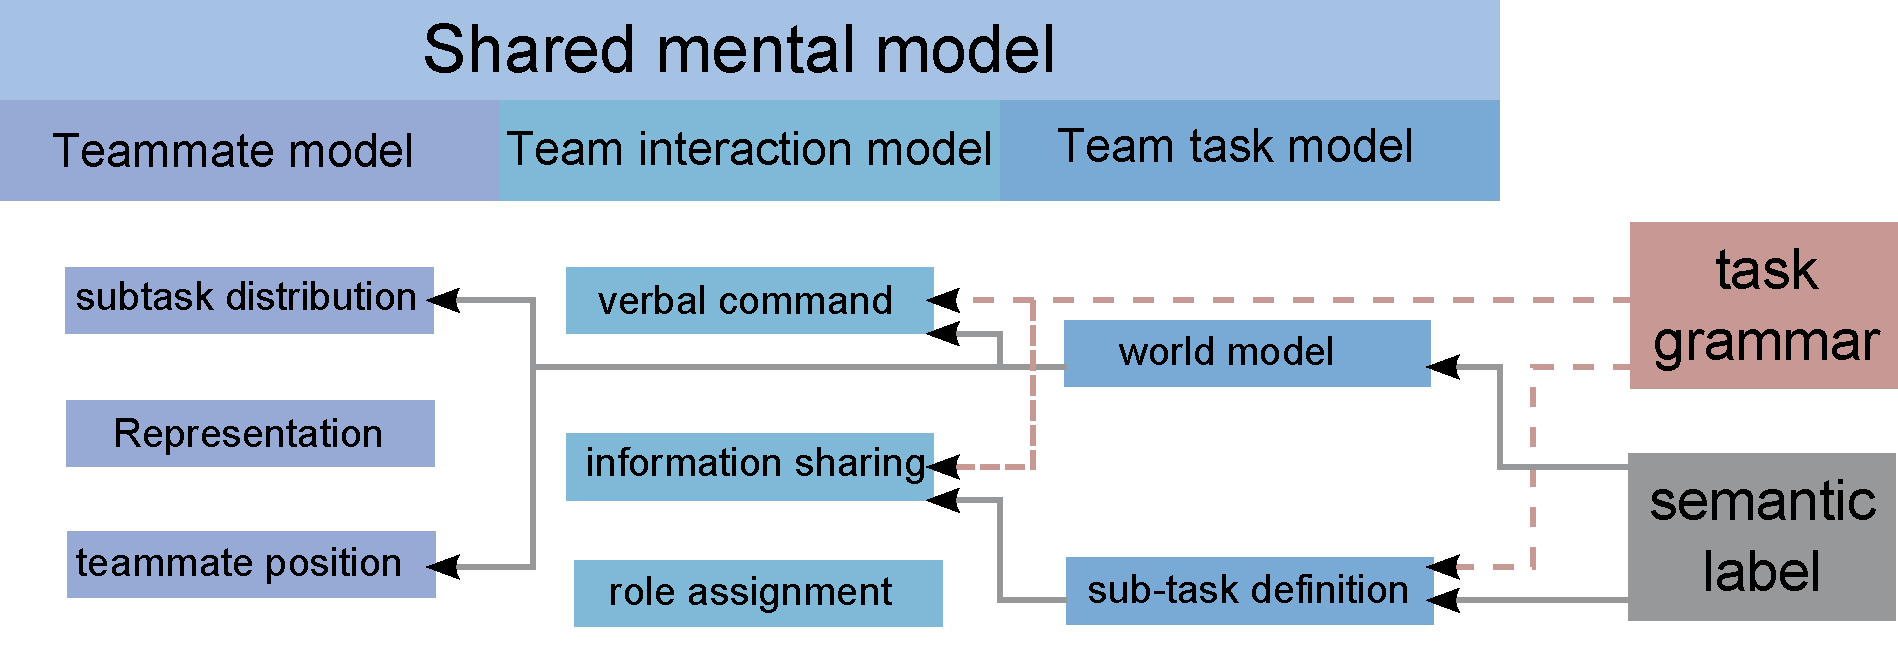
\includegraphics[width=0.7\linewidth]{./images/smm}
\caption{How task grammar and semantic labels support a shared mental model.}
\label{fig:smm}
\end{figure}

A shared mental model of a cordon and search team can be decomposed \cite{goodrich2013toward} into three sub-models.
We list only some elements that are relevant with a cordon and search task as following.
\begin{itemize}
\item
\textbf{A teammate model} provides the knowledge of teammates skills, abilities and tendencies.
\begin{itemize}
\item A \emph{sub-task distribution} indicates how the sub-tasks are assigned to team members.
\item The \emph{teammate positions} indicate the positions of the teammate, localized relative to the spatial semantic objects.
\item The \emph{representation} indicates how the teammate encodes information and problems.
\end{itemize}
\item 
\textbf{A team interaction model} provides the knowledge of roles, responsibilities, information sources, communication channels and role interdependencies.
\begin{itemize}
\item A \emph{role assignment} defines the roles of the members in a team.
\item A \emph{verbal command} describes the format of a command.
\item An \emph{information sharing} represents the information exchange format between team members.
\end{itemize}  
\textbf{A team task model} provides the knowledge of procedures, equipment, situations, constraints.
\begin{itemize}
\item A \emph{semantic world model} is a representation of the workspace with semantic labels.
\item A \emph{sub-task definition} defines the sub-tasks and its objectives.
\end{itemize}
\end{itemize}

Figure \ref{fig:smm} illustrates how these elements in a shared mental model depend on the task grammar and the semantic labels.
The task grammar and semantic labels support the world model and the sub-task definitions.
The world model and the sub-task definitions can then be used to generate verbal commands and help information sharing.
%Also the semantics in the world model can also help to describe how the sub-tasks are distributed to team members and the positions of the teammates in task execution.

Consider the cordon and search for a human-robot team in an urban area.
The labeling process is run before the cordon and search starts. 
Semantic labels are assigned to the sub-regions and the objects in the map.
Supplementary information can be attached to expand the support to different tasks.
We also expect that semantic labels are used to support a more flexible grammar.
We categorize the labels into three types.
\begin{itemize} 
\item \textbf{Indoor} 
The ``indoor'' label defines the region of an indoor environment in the search space.
\item \textbf{Outdoor} 
The ``outdoor'' label defines the region of an outdoor environment in the search space.
There are several sub-types on an outdoor label.
For the purpose of this paper, we consider only three.
\begin{itemize} 
\item \emph{market}: 
The ``market'' label usually defines sources of information, where there is high probability of interested events occurring.
\item \emph{risky}: 
The ``risky'' label indicates potential risks by prior knowledge. 
This implies that these regions have potential risks, which will be considered when safety is an objective in path planning.
\item \emph{unknown}: 
We usually consider unlabeled regions as ``unknown'' by default, which indicates the lack of prior information.
Thus, there is nothing special to be noticed in these regions.
\end{itemize}
\item \textbf{Feature} 
The ``feature'' label defines the objects in the search space.
They can be used for objects of interest, location indicators and etc.
%This will be used for 
There are two types of feature labels, which are
\begin{itemize} 
\item \emph{2D}: ``2D'' label defines the objects on the ground.
\item \emph{2.5D}: ``2.5D'' label defines the objects on the walls of the architectures.
\end{itemize}
\end{itemize}

Figure \ref{fig:Label} illustrates possible semantic labels for a notional world.

\begin{figure}[tbph]
\centering
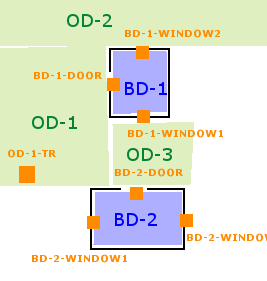
\includegraphics[width=0.4\linewidth]{./images/newLabel-text}
\caption{A labeled map of an urban environment.}
\label{fig:Label}
\end{figure}

Given the semantic labels of a spatial world model, we can define a task grammar by the characteristics of the sub-tasks.
We assume a task grammar that specifies a task, one or more constraints, and one or more adverbs that specify how the task should be performed or how the constraints should be managed.
Equation \ref{eq:task_grammar} is an example of a task grammar that is used in a cordon and search task.
\begin{equation}
\label{eq:task_grammar}
\begin{aligned}
< Start > \rightarrow & < CommandPhrase > \\
< CommandPhrase > \rightarrow & < ScreenCommand > \mid < ProceedCommand > \\
< ScreenCommand > \rightarrow & < Adverb > \mbox{ Screen the } < FeatureQuantifier > < Feature > \mbox{ of the } \\
& < BlockId > \\
< ProceedCommand > \rightarrow & \mbox{ Proceed } < Adverb > < PrepPhrase > \mbox{ to the } < FeatureQuantifier > \\ 
& < Feature >  \mbox{ of the } < BlockId > \\
< Adverb > \rightarrow & \mbox{ covertly } \mid \mbox{ safely } \mid \mbox{ quickly } \mid \mbox{carefully}\\
<FeatureQuantifier> \rightarrow & \mbox{ back }  \mid \mbox { front } \mid \mbox{ side } \\
<Feature> \rightarrow & \mbox{ door } \mid \mbox{ window } \mid \mbox{ exits } \\
<BlockType> \rightarrow & \mbox{ BD- } \mid \mbox{ OB- } \\
<PrepPhrase> \rightarrow & < PrepSegment > \mbox{ the } < BlockId > \mid \mbox{ between the } < BlockId > \\
& \mbox{ and the } < BlockId > \\
< BlockId > \rightarrow & < BlockType > < Id > \\
<PrepSegment> \rightarrow & \mbox{ around } \mid \mbox{ left-of } \mid \mbox{ right-of }
\end{aligned}
\end{equation}

For example, if a human tells a robot to ``carefully screen the OB-2'', this command defines a sub-task as a ``screen'' action.
``OB-2'' is a semantic label, which constrains the task to specific work region.
Besides what to do in a sub-task, this verbal command also implies how to evaluate the performance of this sub-task.
Some of the objectives inherit from the properties of a screen action,
the other objectives are from the adverb, e.g. ``carefully''.
This turns the path-planning problem in the sub-task into a multi-objective optimization problem as described in the next section.
